\documentclass{standalone}
\usepackage[utf8]{inputenc}
\usepackage{tikz}
\usetikzlibrary{shapes.geometric, arrows, positioning, fit, backgrounds, calc}
\usepackage{helvet}
\renewcommand{\familydefault}{\sfdefault}

\begin{document}
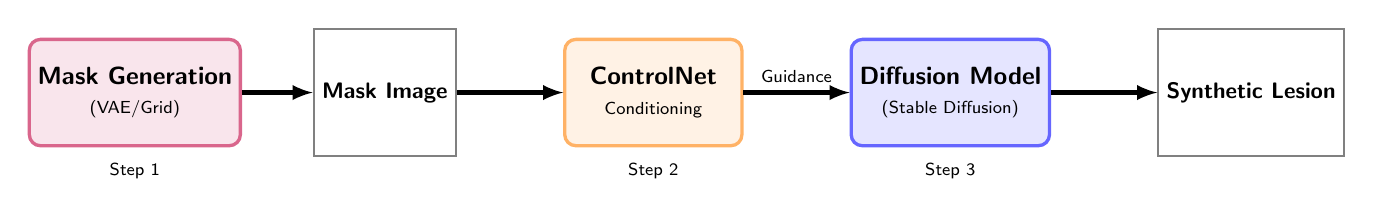
\begin{tikzpicture}[
    node distance=1.5cm,
    auto,
    scale=0.9,
    transform shape,
    box/.style={rectangle, rounded corners, minimum width=2.5cm, minimum height=1.5cm, align=center, draw=black!70, very thick, font=\sffamily},
    maskstep/.style={box, fill=purple!10, draw=purple!60},
    controlstep/.style={box, fill=orange!10, draw=orange!60},
    genstep/.style={box, fill=blue!10, draw=blue!60},
    image/.style={rectangle, minimum size=1.8cm, align=center, draw=black!50, fill=white, thick, font=\sffamily\small},
    arrow/.style={-latex, thick, line width=1.5pt}
]

    % Step 1: Mask
    \node[maskstep] (mask_gen) {\textbf{Mask Generation}\\\scriptsize (VAE/Grid)};
    \node[image, right=1cm of mask_gen] (mask_img) {\textbf{Mask Image}};
    
    % Step 2: ControlNet
    \node[controlstep, right=1.5cm of mask_img] (controlnet) {\textbf{ControlNet}\\\scriptsize Conditioning};
    
    % Step 3: Generation
    \node[genstep, right=1.5cm of controlnet] (diffusion) {\textbf{Diffusion Model}\\\scriptsize (Stable Diffusion)};
    
    % Output
    \node[image, right=1.5cm of diffusion] (output) {\textbf{Synthetic Lesion}};

    % Connections
    \draw[arrow] (mask_gen) -- (mask_img);
    \draw[arrow] (mask_img) -- (controlnet);
    \draw[arrow] (controlnet) -- node[above] {\scriptsize Guidance} (diffusion);
    \draw[arrow] (diffusion) -- (output);
    
    % Annotations
    \node[below=0.1cm of mask_gen] {\scriptsize Step 1};
    \node[below=0.1cm of controlnet] {\scriptsize Step 2};
    \node[below=0.1cm of diffusion] {\scriptsize Step 3};

\end{tikzpicture}
\end{document}
